\documentclass[11pt,onecolumn]{article}
\usepackage[letterpaper,margin=1in]{geometry}
\usepackage[document]{ragged2e}               % ragged right alignment
\usepackage{mathpazo}                         % Palatino font
\usepackage[T1]{fontenc}                      % some font encoding stuff
\usepackage{fancyhdr}                         % for nice headers and footers
\usepackage{lastpage}                         % to enable "Page 1 of X"
\usepackage{xcolor}                           % for colors
\usepackage{titlesec}                         % for section title spacing
\usepackage{url}                              % for urls
\usepackage{hyperref}
\usepackage{amsmath}
\usepackage{enumitem}
\usepackage{graphicx}
\usepackage[font=small]{subcaption}
%\usepackage{apaparencite}
\usepackage{csquotes}
\usepackage{wrapfig,booktabs}
%\usepackage[font=small,bf]{caption}
\usepackage[style=authoryear, maxnames=1, backend=bibtex]{biblatex}
\addbibresource{xstream.bib}

\DeclareMathOperator*{\argmax}{\arg\!\max}

% set up formatting
\setlength{\parindent}{0pt}                   % don't indent paragraphs
\setlength{\parskip}{12pt}                    % space between paragraphs
\setlength{\footskip}{18pt}                   % space between last para/footer
\linespread{1.05}
\titlespacing\section{0pt}{0.25\parskip}{0.25\parskip}
\titlespacing\subsection{0pt}{0.25\parskip}{0.25\parskip}
\titlespacing\subsubsection{0pt}{\parskip}{\parskip}
%\setlength{\bibspacing}{\baselineskip}
\setlist[itemize,enumerate]{topsep=0pt}

\setlength{\columnsep}{24pt}%
\newcommand{\method}{{\sc X-stream}}

\usepackage{mathtools}
\DeclarePairedDelimiter\ceil{\lceil}{\rceil}
\DeclarePairedDelimiter\floor{\lfloor}{\rfloor}

% set up headers and footers
\pagestyle{fancy}
\fancyhf{}
\rfoot{\color{gray}\scriptsize{\thepage \hspace{1pt} of \pageref{LastPage}}}
\lfoot{\color{gray}\scriptsize{XStream -- Emaad Ahmed Manzoor}}
\renewcommand{\headrulewidth}{0pt}

% macros
\definecolor{blue}{HTML}{2b8cbe}
\newcommand{\note}[1]{\textcolor{blue}{#1}}
\newcommand{\R}{\mathbb{R}}

\begin{document}

\textbf{\huge{XStream-Static Temporary}}

\section{Static Dataset Evaluation}

\begin{table}[h!]
	\centering
	\begin{tabular}{lccc}
	\toprule
	\textbf{Dataset} & \textbf{Number of samples} & \textbf{Dimensionality} & \textbf{Number of Anomalies}\\
	\midrule
	\multicolumn{4}{c}{\textit{High-dimensional Datasets}}\\
	gisette 		& 3850 & 4970 & 351	\\
	isolet 			& 4886 & 617 & 389	\\
	letter			& 4586 & 617 & 389	\\
	madelon 		& 1430 & 500 & 130	\\
	\midrule
	\multicolumn{4}{c}{\textit{Low/medium-dimensional Datasets}}\\
	cancer 			& 385      & 30  & 28	\\
	ionosphere  & 242      & 33  & 17		\\
	telescope   & 13283    & 10  & 	951		\\
	indians    	& 538      & 8	& 38		\\
	\bottomrule
	\end{tabular}
	\caption{Datasets used for the static evaluation.}
	\label{table:datasets}
\end{table}

\begin{footnotesize}
\begin{table}[!hbtp]
		\begin{tabular}{lcccccc}
		\toprule
		\textbf{Dataset} & \textbf{IF} &  \textbf{HST} & \textbf{RSH} &  \textbf{LODA}  & \textbf{XS}\\
		\midrule
				\multicolumn{6}{c}{\textit{Original Datasets}}\\
cancer & $0.617 \pm 0.021$ &  $0.646 \pm 0.033$ &  $0.619 \pm 0.03$ &  $0.826 \pm 0.013$  & $0.845 \pm 0.008$    \\
ionosphere& $0.705 \pm 0.006$ &  $0.706 \pm 0.007$ &  $0.764 \pm 0.032$ &  $0.642 \pm 0.067$ & $0.848 \pm 0.018$    \\
telescope& $0.367 \pm 0.008$ &  $0.392 \pm 0.012$ &  $0.391 \pm 0.012$ &  $0.322 \pm 0.007$ & $0.344 \pm 0.009$    \\
indians& $0.142 \pm 0.003$ &  $0.146 \pm 0.002$ &  $0.156 \pm 0.007$ &  $0.177 \pm 0.008$ & $0.216 \pm 0.01$    \\
gisette& $0.078 \pm 0.002$ &  $0.08 \pm 0.002$ &  $0.084 \pm 0.007$ &  $0.087 \pm 0.003$ & $0.09 \pm 0.003$    \\
isolet& $0.099 \pm 0.003$ &  $0.097 \pm 0.005$ &  $0.108 \pm 0.004$ &  $0.089 \pm 0.004$ & $0.112 \pm 0.006$    \\
letter-recognition& $0.093 \pm 0.001$ &  $0.092 \pm 0.002$ &  $0.104 \pm 0.004$ &  $0.094 \pm 0.006$ & $0.122 \pm 0.005$    \\
madelon& $0.11 \pm 0.003$ &  $0.101 \pm 0.013$ &  $0.092 \pm 0.005$ &  $0.101 \pm 0.01$ & $0.097 \pm 0.004$    \\
		\bottomrule
		\end{tabular}
		\caption{Average precision of static methods on original, unperturbed datasets. Mean and standard deviation are reported over 10 runs.}
\end{table}
\end{footnotesize}

\begin{footnotesize}
\begin{table}[p!]
    %\centering
		\begin{tabular}{lcccccc}
				\toprule
				\textbf{Dataset} & \textbf{IF} &  \textbf{HST} & \textbf{RSH} &  \textbf{LODA}  & \textbf{XS}\\
\toprule
cancer(100.0,0.1 )& $0.599 \pm 0.031$ &  $0.605 \pm 0.031$ &  $0.646 \pm 0.032$ &  $0.811 \pm 0.012$ &  $0.825 \pm 0.012$    \\
cancer(1000.0,0.1 )& $0.406 \pm 0.088$ &  $0.201 \pm 0.024$ &  $0.425 \pm 0.112$ &  $0.722 \pm 0.056$ &  $0.813 \pm 0.022$    \\
cancer(2000.0,0.1 )& $0.306 \pm 0.044$ &  $0.229 \pm 0.029$ &  $0.337 \pm 0.077$ &  $0.633 \pm 0.092$ &  $0.822 \pm 0.021$    \\
cancer(5000.0,0.1 )& $0.12 \pm 0.04$ &  $0.158 \pm 0.018$ &  $0.153 \pm 0.07$ &  $0.336 \pm 0.141$ &  $0.796 \pm 0.028$    \\
\midrule
ionosphere (100.0,0.1 )& $0.651 \pm 0.049$ &  $0.568 \pm 0.026$ &  $0.622 \pm 0.038$ &  $0.56 \pm 0.056$ &  $0.848 \pm 0.011$    \\
ionosphere (1000.0,0.1 )& $0.302 \pm 0.072$ &  $0.231 \pm 0.006$ &  $0.258 \pm 0.07$ &  $0.589 \pm 0.073$ &  $0.819 \pm 0.019$    \\
ionosphere (2000.0,0.1 )& $0.211 \pm 0.105$ &  $0.085 \pm 0.007$ &  $0.233 \pm 0.1$ &  $0.561 \pm 0.092$ &  $0.791 \pm 0.026$    \\
ionosphere (5000.0,0.1 )& $0.112 \pm 0.035$ &  $0.15 \pm 0.017$ &  $0.135 \pm 0.062$ &  $0.494 \pm 0.072$ &  $0.685 \pm 0.065$    \\
\midrule
telescope (100.0,0.1 )& $0.311 \pm 0.012$ &  $0.26 \pm 0.006$ &  $0.326 \pm 0.015$ &  $0.322 \pm 0.006$ &  $0.34 \pm 0.008$    \\
telescope (1000.0,0.1 )& $0.156 \pm 0.011$ &  $0.102 \pm 0.004$ &  $0.164 \pm 0.019$ &  $0.303 \pm 0.01$ &  $0.311 \pm 0.006$    \\
telescope (2000.0,0.1 )& $0.108 \pm 0.01$ &  $0.098 \pm 0.014$ &  $0.112 \pm 0.019$ &  $0.296 \pm 0.016$ &  $0.284 \pm 0.005$    \\
telescope (5000.0,0.1 )& $0.084 \pm 0.005$ &  $0.079 \pm 0.001$ &  $0.087 \pm 0.011$ &  $0.248 \pm 0.017$ &  $0.271 \pm 0.005$    \\
\midrule
indians (100.0,0.1 )& $0.123 \pm 0.007$ &  $0.093 \pm 0.003$ &  $0.128 \pm 0.009$ &  $0.171 \pm 0.008$ &  $0.196 \pm 0.015$    \\
indians (1000.0,0.1 )& $0.086 \pm 0.014$ &  $0.096 \pm 0.009$ &  $0.087 \pm 0.011$ &  $0.153 \pm 0.028$ &  $0.178 \pm 0.006$    \\
indians (2000.0,0.1 )& $0.087 \pm 0.013$ &  $0.076 \pm 0.003$ &  $0.085 \pm 0.008$ &  $0.139 \pm 0.028$ &  $0.151 \pm 0.013$    \\
indians (5000.0,0.1 )& $0.073 \pm 0.007$ &  $0.075 \pm 0.009$ &  $0.083 \pm 0.018$ &  $0.126 \pm 0.028$ &  $0.152 \pm 0.02$    \\
				\bottomrule
		\end{tabular}
		\caption{Average precision of static methods on perturbed noisy datasets. Mean and standard deviation reported over 10 runs. Numbers in the brackets indicate: noise column amount (as $\%$ of original dimensionality), relative noise factor.}
		\label{table:static-results}
\end{table}
\end{footnotesize}

We conduct our experiments on datasets mentioned in Table~\ref{table:datasets}. A Friedman test for differences in the best-performing method across all datasets, showed that we cannot reject the null hypothesis that the difference rankings between methods is statistically significant with $p=0.1107$. 

We did perform a posthoc-Friedman test, Nemenyi test to compare all methods to each other. We first compute average ranks of all the methods over the  $8$ original datasets, which is shown in Table~\ref{table:OriginalRanks}. Setting significance level to be $\alpha=0.05$, we get the $q_{0.05}$ for $k=5$ methods as $2.728$. Difference in average ranks of any two methods will be significant if 
\begin{align}
(R_{i} - R_{j}) > q_{\alpha} \sqrt{\frac{k(k+1)}{6N}}
\end{align}
Setting $N=8$ and $k=5$, for difference between a pair of methods to be significant, the difference between the rank should be greater than $2.1567$. Looking at the average ranks shown in Table~\ref{table:OriginalRanks}, we notice that X-Stream has the best ranking on average although no pairs that are significantly different from each other. 

\begin{table}
    \centering
    \begin{tabular}{llllll}
    \toprule
                            & IF         & HST        & RSH        & LODA       & XS          \\	\hline
    cancer & 0.617(5.0) & 0.646(3.0) & 0.619(4.0) & 0.826(2.0) & 0.845(1.0) \\
    ionosphere              & 0.705(4.0) & 0.706(3.0) & 0.764(2.0) & 0.642(5.0) & 0.848(1.0) \\
    magic-telescope         & 0.367(3.0) & 0.392(1.0) & 0.391(2.0) & 0.322(5.0) & 0.344(4.0)  \\
    pima-indians            & 0.142(5.0) & 0.146(4.0) & 0.156(3.0) & 0.177(2.0) & 0.216(1.0) \\
    gisette                 & 0.078(5.0) & 0.08(4.0)  & 0.084(3.0) & 0.087(2.0) & 0.09(1.0) \\
    isolet                  & 0.099(3.0) & 0.097(4.0) & 0.108(2.0) & 0.089(5.0) & 0.112(1.0) \\
    letter-recognition      & 0.093(4.0) & 0.092(5.0) & 0.104(2.0) & 0.094(3.0) & 0.122(1.0) \\
    madelon                 & 0.11(1.0)  & 0.101(2.5) & 0.092(5.0) & 0.101(2.5) & 0.097(4.0) \\
    \midrule
    Avg Rank                & 3.75       & 3.3125     & 2.875      & 3.3125     & 1.75        \\
    \bottomrule
    \end{tabular}
    \caption{Average rank of method over 8 original datasets.}
    \label{table:OriginalRanks}
\end{table}

To show the effect of increasing high-dimensionality, we add noisy columns to the $4$ original datasets. The noise is generated as mentioned above in Approach 1. The average ranks for all the methods is shown in Table~\ref{table:LowDimRanks}. Using Friedman test, we can reject the null hypothesis that the difference in rankings between methods is not statistically significant with $p=5.565\times 10^{-10}$. We again perform posthoc-Friedman Nemenyi test; setting $N=16$ and $k=5$, we obtain that difference in average ranks should be greater than $1.524$. Observing the table, we find difference to be significant between (LODA, I-Forest), (X-Stream, I-Forest), (LODA, HS-Trees), (X-Stream, HS-Trees) and (X-Stream, RS-Hash).

\begin{table}
\centering
    \begin{tabular}{llllll}
    \toprule
                  & IF         & HST        & RSH        & LODA       & XS          \\	\hline
    cancer100     & 0.599(5.0) & 0.605(4.0) & 0.646(3.0) & 0.811(2.0) & 0.825(1.0) \\
    cancer1000    & 0.406(4.0) & 0.201(5.0) & 0.425(3.0) & 0.722(2.0) & 0.813(1.0)  \\
    cancer2000    & 0.306(4.0) & 0.229(5.0) & 0.337(3.0) & 0.633(2.0) & 0.822(1.0) \\
    cancer5000    & 0.12(5.0)  & 0.158(3.0) & 0.153(4.0) & 0.336(2.0) & 0.796(1.0) \\
    ionos100      & 0.651(2.0) & 0.568(4.0) & 0.622(3.0) & 0.56(5.0)  & 0.848(1.0) \\
    ionos1000     & 0.302(3.0) & 0.231(5.0) & 0.258(4.0) & 0.589(2.0) & 0.819(1.0) \\
    ionos2000     & 0.211(4.0) & 0.085(5.0) & 0.233(3.0) & 0.561(2.0) & 0.791(1.0) \\
    ionos5000     & 0.112(5.0) & 0.15(3.0)  & 0.135(4.0) & 0.494(2.0) & 0.685(1.0) \\
    telescope100  & 0.311(4.0) & 0.26(5.0)  & 0.326(2.0) & 0.322(3.0) & 0.34(1.0) \\
    telescope1000 & 0.156(4.0) & 0.102(5.0) & 0.164(3.0) & 0.303(2.0) & 0.311(1.0) \\
    telescope2000 & 0.108(4.0) & 0.098(5.0) & 0.112(3.0) & 0.296(1.0) & 0.284(2.0)  \\
    telescope5000 & 0.084(4.0) & 0.079(5.0) & 0.087(3.0) & 0.248(2.0) & 0.271(1.0) \\
    indians100    & 0.123(4.0) & 0.093(5.0) & 0.128(3.0) & 0.171(2.0) & 0.196(1.0) \\
    indians1000   & 0.086(5.0) & 0.096(3.0) & 0.087(4.0) & 0.153(2.0) & 0.178(1.0) \\
    indians2000   & 0.087(3.0) & 0.076(5.0) & 0.085(4.0) & 0.139(2.0) & 0.151(1.0) \\
    indians5000   & 0.073(5.0) & 0.075(4.0) & 0.083(3.0) & 0.126(2.0) & 0.152(1.0) \\
    \midrule
    Avg Rank      & 4.0625     & 4.4375     & 3.25       & 2.1875     & 1.0625      \\
    \bottomrule
    \end{tabular}
    \caption{Average rank of methods over the 16 perturbed datasets.}
    \label{table:LowDimRanks}
\end{table}

Another form of presenting this could be the visualization, which we present below in Fig~\ref{fig:Nemenyi}.

\begin{figure*}[ht!]
    \centering
    \begin{subfigure}[t]{0.49\textwidth}
        \centering
        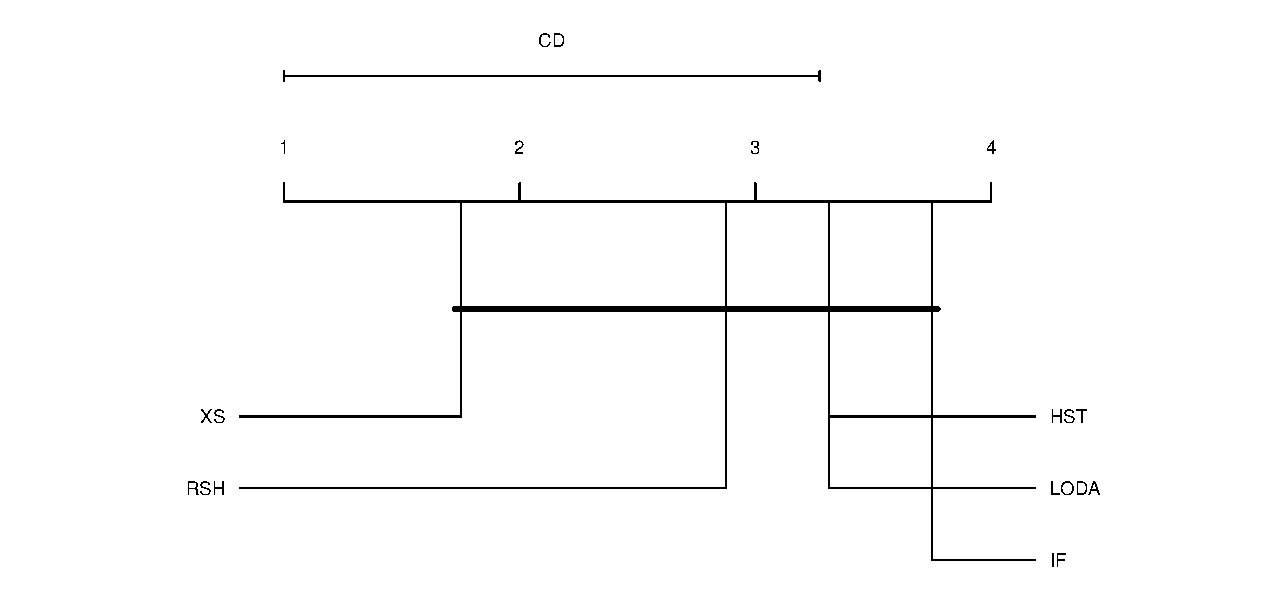
\includegraphics[width=\linewidth]{fig/Nemenyi_Overall.pdf}
        \caption{Nemenyi Test visualization for 8 original datasets.}
    \end{subfigure}
    \hfill
    \begin{subfigure}[t]{0.49\textwidth}
        \centering
        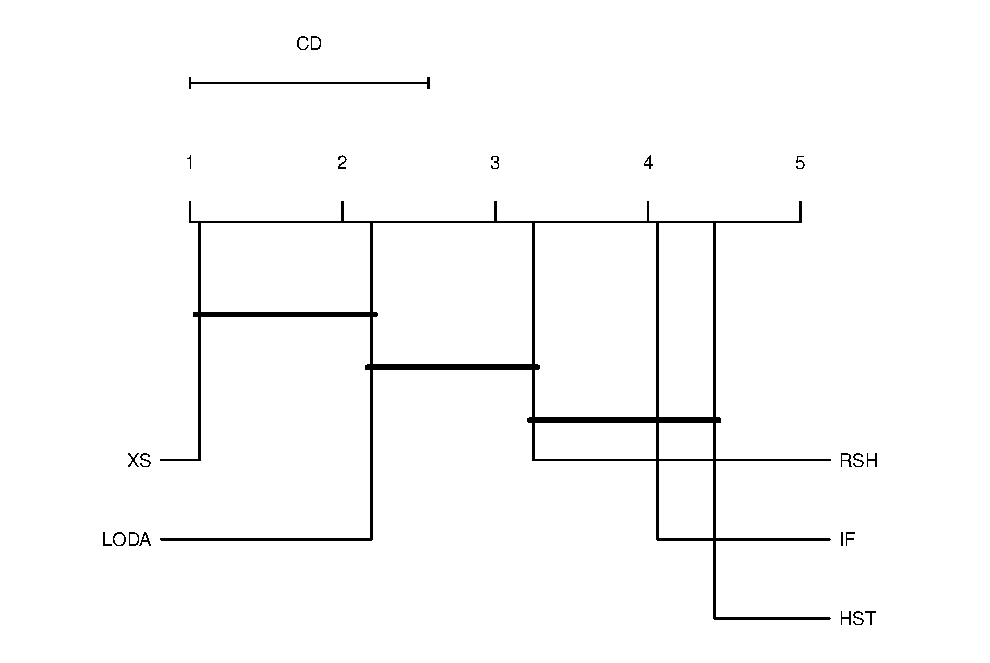
\includegraphics[width=\linewidth]{fig/Nemenyi_LowDim.pdf}
        \caption{Nemenyi Test for 16 perturbed datasets.}
    \end{subfigure}
		\hfill
    \caption{Nemenyi Test Visualization}
    \label{fig:Nemenyi}
\end{figure*}


\section{Alternative Dataset from ODDS}
For evaluating our static approach, we compared the proposed method with four other baseline methods - iForest, LODA, RS-Hash and HS-Trees over 13 datasets we obtained from ODDS repository~\cite{ODDS}.
The list of datasets used and their properties is shown in Table~\ref{table:datasets}.

\begin{table}[h!]
	\centering
	\begin{tabular}{lcccc}
	\toprule
	\textbf{Dataset} & \textbf{Number of samples} & \textbf{Dimensionality} & \textbf{Number of Anomalies} & \textbf{Anomaly Rate}	\\
	\midrule
	annthyroid & 7200 & 6 & 534 & $7.4	\%$\\
	arrhythmia & 452 & 274 & 66 & $14.6\%$\\
	breastw & 683 & 9 & 239 & $34.99\%$\\
	cardio & 1831 & 21 & 176 & $9.6\%$\\
	glass & 214 & 9 & 9 & $4.2\%$\\
	ionosphere & 351 & 33 & 126 & $35.89\%$\\
	lympho & 148 & 18 & 6 & $4.05\%$\\
	pendigits & 6870 & 16 & 156 & $2.27\%$\\
	thyroid & 3772 & 6 & 93 & $2.46\%$\\
	vertebral & 240 & 6 & 30 & $12.5\%$\\
	{vowels} & 1456 & 12 & 50 & $3.43\%$\\
	wbc & 378 & 30 & 21 & $5.55\%$\\
	wine & 129 & 13 & 10 & $7.75\%$\\
	\bottomrule
	\end{tabular}
	\caption{Datasets from ODDS.}
	\label{table:datasets}
\end{table}

\begin{footnotesize}
\begin{table}[p!]
    %\centering
		\begin{tabular}{lcccccc}
				\toprule
				\textbf{Dataset} & \textbf{IF} &  \textbf{HST} & \textbf{RSH} &  \textbf{LODA}  & \textbf{XS}\\
\toprule
annthyroid& $0.312 \pm 0.025$ &  $0.147 \pm 0.004$ &  $0.19 \pm 0.016$ &  $0.196 \pm 0.023$ &  $0.161 \pm 0.012$    \\
arrhythmia& $0.462 \pm 0.009$ &  $0.458 \pm 0.006$ &  $0.467 \pm 0.023$ &  $0.496 \pm 0.029$ &  $0.494 \pm 0.014$    \\
breastw& $0.948 \pm 0.008$ &  $0.98 \pm 0.003$ &  $0.967 \pm 0.003$ &  $0.966 \pm 0.005$ &  $0.96 \pm 0.005$    \\
cardio& $0.538 \pm 0.044$ &  $0.681 \pm 0.006$ &  $0.522 \pm 0.034$ &  $0.523 \pm 0.041$ &  $0.504 \pm 0.015$    \\
glass& $0.082 \pm 0.009$ &  $0.092 \pm 0.004$ &  $0.089 \pm 0.008$ &  $0.116 \pm 0.03$ &  $0.129 \pm 0.024$    \\
ionosphere& $0.822 \pm 0.006$ &  $0.822 \pm 0.002$ &  $0.824 \pm 0.013$ &  $0.78 \pm 0.024$ &  $0.888 \pm 0.006$    \\
lympho& $0.948 \pm 0.036$ &  $0.99 \pm 0.013$ &  $0.967 \pm 0.033$ &  $0.919 \pm 0.067$ &  $0.581 \pm 0.063$    \\
pendigits& $0.275 \pm 0.029$ &  $0.266 \pm 0.03$ &  $0.23 \pm 0.021$ &  $0.27 \pm 0.074$ &  $0.147 \pm 0.014$    \\
thyroid& $0.554 \pm 0.035$ &  $0.228 \pm 0.007$ &  $0.299 \pm 0.024$ &  $0.253 \pm 0.042$ &  $0.183 \pm 0.019$    \\
vertebral& $0.093 \pm 0.002$ &  $0.081 \pm 0.001$ &  $0.086 \pm 0.002$ &  $0.084 \pm 0.002$ &  $0.087 \pm 0.003$    \\
vowels& $0.176 \pm 0.056$ &  $0.162 \pm 0.006$ &  $0.211 \pm 0.044$ &  $0.115 \pm 0.044$ &  $0.398 \pm 0.034$    \\
wbc& $0.594 \pm 0.025$ &  $0.582 \pm 0.01$ &  $0.597 \pm 0.02$ &  $0.591 \pm 0.039$ &  $0.437 \pm 0.034$    \\
wine& $0.174 \pm 0.023$ &  $0.186 \pm 0.014$ &  $0.209 \pm 0.015$ &  $0.588 \pm 0.134$ &  $0.252 \pm 0.033$    \\
\bottomrule
		\end{tabular}
		\caption{Average precision of static methods on dataset from ODDS. Mean and standard deviation reported over 10 runs.}
		\label{table:odds-static-results}
\end{table}
\end{footnotesize}

\begin{table}
	\centering
    \begin{tabular}{llllll}
    \toprule
                     & IF          & HST         & RSH         & LODA        & XS          \\	\hline
    annthyroid & 0.312(1.0)  & 0.147(5.0)  & 0.19(3.0)   & 0.196(2.0)  & 0.161(4.0) \\
    arrhythmia & 0.462(4.0)  & 0.458(5.0)  & 0.467(3.0)  & 0.496(1.0)  & 0.494(2.0) \\
    breastw    & 0.948(5.0)  & 0.98(1.0)   & 0.967(2.0)  & 0.966(3.0)  & 0.96(4.0) \\
    cardio     & 0.538(2.0)  & 0.681(1.0)  & 0.522(4.0)  & 0.523(3.0)  & 0.504(5.0) \\
    glass      & 0.082(5.0)  & 0.092(3.0)  & 0.089(4.0)  & 0.116(2.0)  & 0.129(1.0) \\
    ionosphere & 0.822(3.5)  & 0.822(3.5)  & 0.824(2.0)  & 0.78(5.0)   & 0.888(1.0) \\
    lympho     & 0.948(3.0)  & 0.99(1.0)   & 0.967(2.0)  & 0.919(4.0)  & 0.581(5.0) \\
    pendigits  & 0.275(1.0)  & 0.266(3.0)  & 0.23(4.0)   & 0.27(2.0)   & 0.147(5.0) \\
    thyroid   & 0.554(1.0)  & 0.228(4.0)  & 0.299(2.0)  & 0.253(3.0)  & 0.183(5.0) \\
    vertebral  & 0.093(1.0)  & 0.081(5.0)  & 0.086(3.0)  & 0.084(4.0)  & 0.087(2.0) \\
    vowels     & 0.176(3.0)  & 0.162(4.0)  & 0.211(2.0)  & 0.115(5.0)  & 0.398(1.0) \\
    wbc        & 0.594(2.0)  & 0.582(4.0)  & 0.597(1.0)  & 0.591(3.0)  & 0.437(5.0) \\
    wine       & 0.174(5.0)  & 0.186(4.0)  & 0.209(3.0)  & 0.588(1.0)  & 0.252(2.0) \\
    \midrule
    Avg Rank         & 2.807  & 3.346  & 2.692  & 2.923  & 3.23  \\
    \bottomrule
    \end{tabular}
    \caption{Average rank of methods over the 13 ODDS datasets.}
    \label{table:odds-static-rank}
\end{table}

A Friedman test for differences in the best-performing method across all datasets, showed that we cannot reject the null hypothesis that the difference rankings between methods is NOT statistically significant with $p=0.8049$. We did perform a posthoc-Friedman test, Nemenyi test to compare all methods to each other. We first compute average ranks of all the methods over the  $13$ datasets, which is shown in Table~\ref{table:odds-static-rank}. Setting $N=13$ and $k=5$, we obtain that difference in average ranks should be greater than $1.692$. We can see that difference between none of the pairs is significant. Therefore, we can safely say that on standard datasets, all the methods are similar.

\begin{figure*}[ht!]
    \centering
%    \begin{subfigure}[t]{0.49\textwidth}
        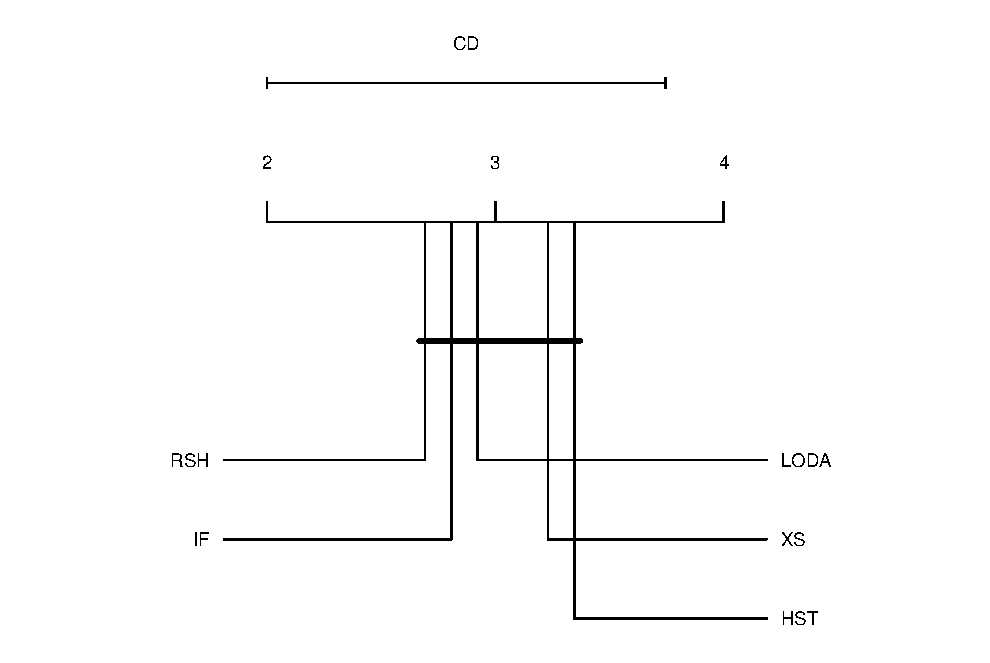
\includegraphics[width=\linewidth]{fig/Nemenyi_ODDS_All.pdf}
%    \end{subfigure}
%    \hfill
        \caption{Nemenyi Test visualization for 13 original datasets from ODDS.}
    \label{fig:Nemenyi-ODDS-ALL}
\end{figure*}

\textbf{Distorting ODDS datasets}

To study the effect of adding noisy columns and high-dimensionality in datasets, we choose to distort by adding noisy columns only to the datasets for which all $5$ methods are performing reasonably well i.e. breastw, cardio, ionosphere and lympho. 

\begin{footnotesize}
\begin{table}[p!]
    %\centering
		\begin{tabular}{lcccccc}
				\toprule
				\textbf{Dataset} & \textbf{IF} &  \textbf{HST} & \textbf{RSH} &  \textbf{LODA}  & \textbf{XS}\\
\toprule
breastw (1000,0.1 )& $0.789 \pm 0.028$ &  $0.841 \pm 0.024$ &  $0.782 \pm 0.03$ &  $0.98 \pm 0.006$ &  $0.967 \pm 0.008$    \\
breastw (2000,0.1 )& $0.649 \pm 0.05$ &  $0.703 \pm 0.024$ &  $0.642 \pm 0.07$ &  $0.966 \pm 0.014$ &  $0.967 \pm 0.004$    \\
breastw (3000,0.1 )& $0.551 \pm 0.041$ &  $0.663 \pm 0.014$ &  $0.566 \pm 0.052$ &  $0.958 \pm 0.013$ &  $0.97 \pm 0.006$    \\
%breastw (4000.0,0.1 )& $0.534 \pm 0.032$ &  $0.581 \pm 0.02$ &  $0.535 \pm 0.073$ &  $0.939 \pm 0.022$ &  $0.9746 \pm 0.0033$    \\
breastw (5000,0.1 )& $0.461 \pm 0.029$ &  $0.626 \pm 0.034$ &  $0.458 \pm 0.054$ &  $0.91 \pm 0.046$ &  $0.971 \pm 0.003$    \\
\midrule
cardio (1000.0,0.1 )& $0.245 \pm 0.029$ &  $0.161 \pm 0.006$ &  $0.226 \pm 0.036$ &  $0.56 \pm 0.043$ &  $0.493 \pm 0.017$    \\
cardio (2000,0.1 )& $0.155 \pm 0.023$ &  $0.133 \pm 0.004$ &  $0.153 \pm 0.027$ &  $0.51 \pm 0.074$ &  $0.508 \pm 0.017$    \\
cardio (3000,0.1 )& $0.136 \pm 0.018$ &  $0.107 \pm 0.006$ &  $0.148 \pm 0.019$ &  $0.484 \pm 0.071$ &  $0.537 \pm 0.016$    \\
%cardio (4000.0,0.1 )& $0.12 \pm 0.012$ &  $0.107 \pm 0.005$ &  $0.115 \pm 0.015$ &  $0.426 \pm 0.054$ &  $0.4836 \pm 0.0234$    \\
cardio (5000,0.1 )& $0.11 \pm 0.007$ &  $0.115 \pm 0.003$ &  $0.108 \pm 0.01$ &  $0.458 \pm 0.073$ &  $0.488 \pm 0.017$    \\
\midrule
ionosphere (1000,0.1 )& $0.58 \pm 0.03$ &  $0.549 \pm 0.022$ &  $0.541 \pm 0.042$ &  $0.735 \pm 0.035$ &  $0.861 \pm 0.007$    \\
ionosphere (2000,0.1 )& $0.515 \pm 0.039$ &  $0.421 \pm 0.004$ &  $0.472 \pm 0.028$ &  $0.707 \pm 0.027$ &  $0.866 \pm 0.009$    \\
ionosphere (3000,0.1 )& $0.439 \pm 0.03$ &  $0.433 \pm 0.015$ &  $0.43 \pm 0.018$ &  $0.704 \pm 0.035$ &  $0.822 \pm 0.009$    \\
%ionosphere (4000.0,0.1 )& $0.428 \pm 0.029$ &  $0.346 \pm 0.007$ &  $0.398 \pm 0.028$ &  $0.677 \pm 0.026$ &  $0.812 \pm 0.0068$    \\
ionosphere (5000,0.1 )& $0.4 \pm 0.031$ &  $0.428 \pm 0.016$ &  $0.395 \pm 0.024$ &  $0.7 \pm 0.028$ &  $0.792 \pm 0.008$    \\
\midrule
lympho (1000,0.1 )& $0.362 \pm 0.16$ &  $0.422 \pm 0.064$ &  $0.287 \pm 0.174$ &  $0.667 \pm 0.115$ &  $0.484 \pm 0.114$    \\
lympho (2000,0.1 )& $0.148 \pm 0.093$ &  $0.057 \pm 0.007$ &  $0.091 \pm 0.073$ &  $0.5 \pm 0.173$ &  $0.321 \pm 0.183$    \\
lympho (3000,0.1 )& $0.189 \pm 0.097$ &  $0.037 \pm 0.003$ &  $0.099 \pm 0.074$ &  $0.47 \pm 0.191$ &  $0.414 \pm 0.154$    \\
%lympho (4000.0,0.1 )& $0.134 \pm 0.08$ &  $0.104 \pm 0.012$ &  $0.059 \pm 0.022$ &  $0.284 \pm 0.109$ &  $0.1973 \pm 0.1099$    \\
lympho (5000,0.1 )& $0.073 \pm 0.056$ &  $0.103 \pm 0.026$ &  $0.065 \pm 0.061$ &  $0.274 \pm 0.203$ &  $0.317 \pm 0.091$    \\
\bottomrule
		\end{tabular}
		\caption{Average precision of static methods on perturbed dataset from ODDS. Mean and standard deviation reported over 10 runs. Numbers in the brackets indicate: noise column amount (as $\%$ of original dimensionality), relative noise factor.}
		\label{table:odds-static-results}
\end{table}
\end{footnotesize}

\begin{table}
	\centering
    \begin{tabular}{llllll}
    \toprule
                         & IF         & HST        & RSH        & LODA       & XS          \\	\hline
    breastw(1000,0.1)    & 0.789(4.0) & 0.841(3.0) & 0.782(5.0) & 0.98(1.0)  & 0.967(2.0) \\
    breastw(2000,0.1)    & 0.649(4.0) & 0.703(3.0) & 0.642(5.0) & 0.966(2.0) & 0.967(1.0) \\
    breastw(3000,0.1)    & 0.551(5.0) & 0.663(3.0) & 0.566(4.0) & 0.958(2.0) & 0.970(1.0) \\
    %breastw(4000,0.1)    & 0.534(5.0) & 0.581(3.0) & 0.535(4.0) & 0.939(2.0) & 0.9746(1.0) \\
    breastw(5000,0.1)    & 0.461(4.0) & 0.626(3.0) & 0.458(5.0) & 0.91(2.0)  & 0.971(1.0) \\
    \midrule
    cardio(1000,0.1)     & 0.245(3.0) & 0.161(5.0) & 0.226(4.0) & 0.56(1.0)  & 0.493(2.0) \\
    cardio(2000,0.1)     & 0.155(3.0) & 0.133(5.0) & 0.153(4.0) & 0.51(1.0)  & 0.508(2.0) \\
    cardio(3000,0.1)     & 0.136(4.0) & 0.107(5.0) & 0.148(3.0) & 0.484(2.0) & 0.537(1.0) \\
    %cardio(4000,0.1)     & 0.12(3.0)  & 0.107(5.0) & 0.115(4.0) & 0.426(2.0) & 0.4836(1.0) \\
    cardio(5000,0.1)     & 0.11(4.0)  & 0.115(3.0) & 0.108(5.0) & 0.458(2.0) & 0.488(1.0) \\
    \midrule
    ionosphere(1000,0.1) & 0.58(3.0)  & 0.549(4.0) & 0.541(5.0) & 0.735(2.0) & 0.861(1.0) \\
    ionosphere(2000,0.1) & 0.515(3.0) & 0.421(5.0) & 0.472(4.0) & 0.707(2.0) & 0.866(1.0) \\
    ionosphere(3000,0.1) & 0.439(3.0) & 0.433(4.0) & 0.43(5.0)  & 0.704(2.0) & 0.822(1.0)  \\
    %ionosphere(4000,0.1) & 0.428(3.0) & 0.346(5.0) & 0.398(4.0) & 0.677(2.0) & 0.812(1.0)  \\
    ionosphere(5000,0.1) & 0.4(4.0)   & 0.428(3.0) & 0.395(5.0) & 0.7(2.0)   & 0.792(1.0) \\
    \midrule
    lympho(1000,0.1)     & 0.362(4.0) & 0.422(3.0) & 0.287(5.0) & 0.667(1.0) & 0.484(2.0) \\
    lympho(2000,0.1)     & 0.148(3.0) & 0.057(5.0) & 0.091(4.0) & 0.5(1.0)   & 0.321(2.0) \\
    lympho(3000,0.1)     & 0.189(3.0) & 0.037(5.0) & 0.099(4.0) & 0.47(1.0)  & 0.414(2.0) \\
    %lympho(4000,0.1)     & 0.134(3.0) & 0.104(4.0) & 0.059(5.0) & 0.284(1.0) & 0.1973(2.0) \\
    lympho(5000,0.1)     & 0.073(4.0) & 0.103(3.0) & 0.065(5.0) & 0.274(2.0) & 0.317(1.0) \\
    \midrule
%    Avg Rank             & 3.6        & 3.95       & 4.45       & 1.65       & 1.35        \\
    Avg Rank		& 3.625	& 3.876	& 4.5 	& 1.625	& 1.375		\\
    \bottomrule
    \end{tabular}
    \caption{Average rank of methods over the 16 perturbed datasets.}
    \label{table:odds-distort-rank}
\end{table}

%We present the results on those $4$ datasets in Table~\ref{table:odds-distort-rank}. Using Friedman test, we can reject the null hypothesis that the difference rankings between methods is not statistically significant with $p=5.925\times 10^{-13}$. We again perform posthoc-Friedman Nemenyi test; setting $N=20$ and $k=5$, we obtain that difference in average ranks should be greater than $1.364$. 
%Observing the table~\ref{table:odds-distort-rank}, we find difference to be significant between (LODA, I-Forest), (X-Stream, I-Forest), (LODA, HS-Trees), (X-Stream, HS-Trees), (LODA, RS-Hash), and (X-Stream, RS-Hash). Though X-Stream is not significantly different from LODA, but the average rank of X-Stream is better than that of LODA. We visualize the same in Fig:~\ref{fig:Nemenyi-ODDS-distort}.

We present the results on those $4$ datasets in Table~\ref{table:odds-distort-rank}. Using Friedman test, we can reject the null hypothesis that the difference rankings between methods is not statistically significant with $p=2.458\times 10^{-10}$. We again perform posthoc-Friedman Nemenyi test; setting $N=16$ and $k=5$, we obtain that difference in average ranks should be greater than $1.524$. 
Observing the table~\ref{table:odds-distort-rank}, we find difference to be significant between (LODA, I-Forest), (X-Stream, I-Forest), (LODA, HS-Trees), (X-Stream, HS-Trees), (LODA, RS-Hash), and (X-Stream, RS-Hash). Though X-Stream is not significantly different from LODA, but the average rank of X-Stream is better than that of LODA. We visualize the same in Fig:~\ref{fig:Nemenyi-ODDS-distort}.

\begin{figure*}[ht!]
    \centering
%    \begin{subfigure}[t]{0.49\textwidth}
        %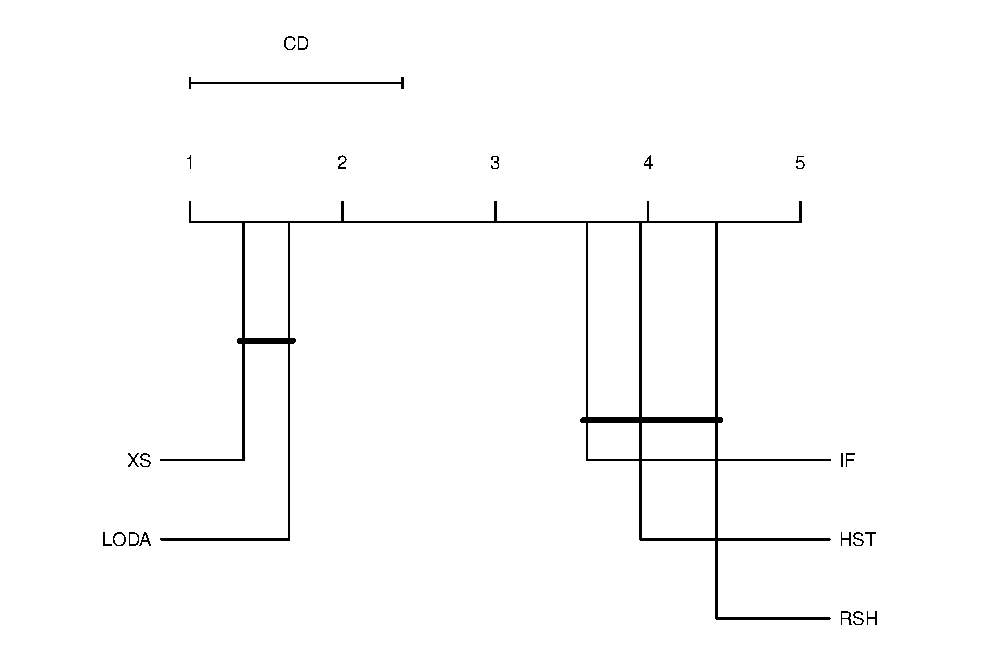
\includegraphics[width=0.7\linewidth]{fig/Nemenyi_Distort.pdf}
        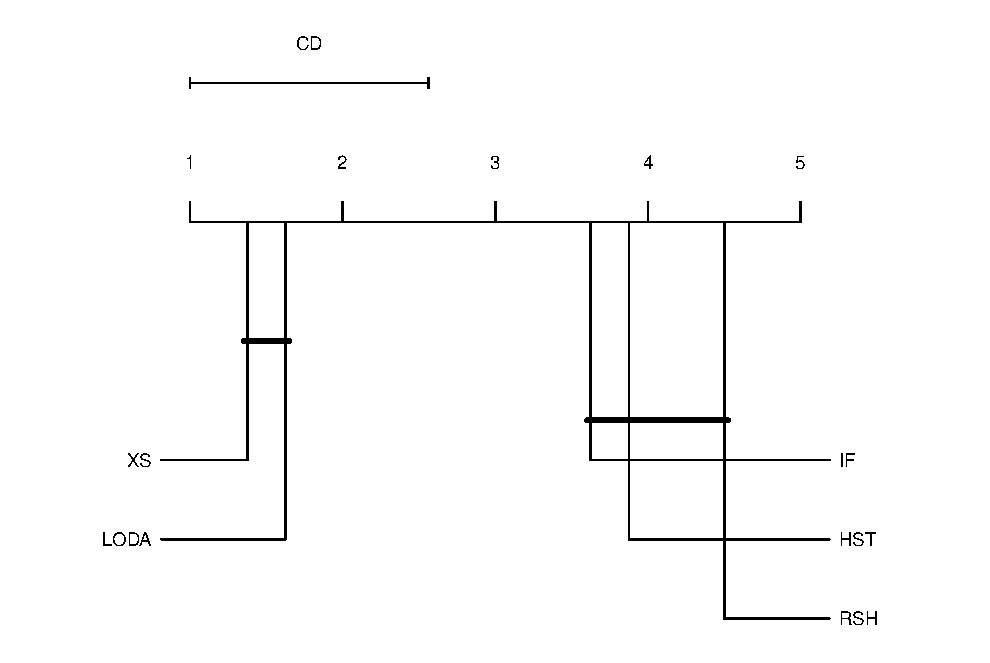
\includegraphics[width=0.7\linewidth]{fig/Nemenyi_Distort_16.pdf}
%    \end{subfigure}
%    \hfill
        \caption{Nemenyi Test visualization for 16 perturbed ODDS datasets.}
    \label{fig:Nemenyi-ODDS-distort}
\end{figure*}


%\section{Combined Datasets}
%We test our approach on the following datasets as listed in Table~\ref{table:combined-datasets}
%\begin{table}[h!]
%	\centering
%	\begin{tabular}{lccc}
%	\toprule
%	\textbf{Dataset} & \textbf{Number of samples} & \textbf{Dimensionality} & \textbf{Number of Anomalies}\\
%	\midrule
%	cancer 			& 385      & 30  & 28	\\
%	ionosphere  & 242      & 33  & 17		\\
%	telescope   & 13283    & 10  & 	951		\\
%	indians    	& 538      & 8	& 38		\\
%	annthyroid & 7200 & 6 & 534 \\
%	arrhythmia & 452 & 274 & 66 \\
%	breastw & 683 & 9 & 239 \\
%	\textbf{cardio} & 1831 & 21 & 176 \\
%	glass & 214 & 9 & 9 \\
%	ionosphere & 351 & 33 & 126 \\
%	\textbf{lympho} & 148 & 18 & 6 \\
%	pendigits & 6870 & 16 & 156 \\
%	thyroid & 3772 & 6 & 93 \\
%	vertebral & 240 & 6 & 30 \\
%	{vowels} & 1456 & 12 & 50 \\
%	\textbf{wbc} & 378 & 30 & 21 \\
%	wine & 129 & 13 & 10 \\
%	\bottomrule
%	\end{tabular}
%	\caption{Datasets from ODDS.}
%	\label{table:combined-datasets}
%\end{table}

%The problem with this is
\printbibliography
\end{document}

